\chapter{\Des}
\inline{sammenligning af simulation vs. modellering.\\
  simulering er en implementation af modellen.\\
  styrke er samspillet mellem flere elementer/modeller.\\
  simulering - dynamisk - tid (time/space).} 

Simuleringer har længe været et værdifuldt værktøj til at klarlægge hvordan et 
system fungerer og er specielt brugbart til at repræsentere systemer hvis 
tilstand ændres over tid, eller såfremt der er interaktion mellem flere systemer. En 
matematisk model af disse systemer vil ofte være væsentligt mere kompleks og 
kan være svær at overskue lige så let som en simulering af samme system. 

Simuleringer foretages ofte af andre videnskabsfolk end dataloger, og det er 
derfor vigtigt at de kan repræsenteres i et sprog som er let tilgængeligt og 
minimerer sandsynligheden for at begå fejl i konstruktionen af simulationen.  
Til dette formål er programmeringssproget Python oplagt da det netop fokuserer 
på let tilgængelighed og høj produktivitet for udvikleren. 

Det er oplagt at benytte CSP\cite{hoare-csp} til at repræsentere en simulering.  
I CSP er interaktionen mellem forskellige processer/systemer eksplicit, og på 
grund af modulariteten er det nemt at konstruere komplekse systemer ud fra 
mindre, enkle systemer. 

\section{Beskrivelse/teori} \label{sec:des-teori}
\inline{Beskrivelse af tidsmodellen, teorien omkring den og hvor/hvad den 
    benyttes til. Teori: henvisning til litteratur, bl.a.  matematik/beviser 
    for modellen}
\inline{Skal vi skrive noget om at introduktionen af tid er det samme som at introducere prioritet}

\begin{shaded}
\fxnote{Gennemlæses og højst sandlysningt omskrives med henblik på sammenhæng og mangler.}
Indenfor simulering er \des en meget brugt metode til at modellere systemer. I 
\des anskues tid som diskrete tidsskridt som er uden kobling til realtid. I 
disse tidsskridt udføres en eller flere begivenheder, som hver især ændrer på systemets tilstand. Når alle begivenheder for et tidsskridt er udført kan tiden tælles op og begivenheder for det nye tidsskridt kan udføres. Der kan være være planlagt et vilkårligt antal beginvenheder til et tidsskridt og hver begivenhed kan variere vilkårligt med henlik på hvor langt tid den tager at udføre i realtid. Det er disse betingelser der forårsager at der ikke er nogen kobling mellem den diskrete tid og realtid, og et diskret tidsskridt kan derved variere arbitrært i realtid. Begivenhederne der skal udføres af systemet kan enten være givet på forhånd, eller blive skemaplanlagt dynamisk under afviklingen af andre begivenheder. 
Afhængig af hvad der simuleres, kan man udtrække relevant information om systemet, f.eks. gennemsnitlig behandlingstid for elementer, længden af køer i systemet, og den samlede aktivitetstid for hvert delelement i systemet.


For at kunne konstruere en \des skal vi have følgende til rådighed; En repræsentation af tid til at styre hvornår vi skifter tidsskridt, en liste over begivenheder der skal udføres i hvert tidsskridt, samt mulighed for at opsamle statistisk data fra simulationen. 

    
I \csp har vi garanti for at de eneste afhængigheder mellem processer vil være kommunikation. I \des har vi ud over kommunikation også en afhængighed af at synkronisere tiden mellem processerne.En simulering løber begivenhederne kronologisk igennem til der enten ikke er flere begivenheder eller som det oftere er tilfældet til simuleringen når et forud defineret tidspunkt.

\fxnote*[inline,nomargin]{Brian: ok brug af parallelitet}{Alternativet til  \des  er \pdes hvor tiden i processerne kan løbe uafhængigt af hinanden. Dette introducerer muligheden for større parallitet, men samtidigt risikerer processerne ved kommunikation at modtage beskeder fra fortiden, som der skal tages hånd om, f.eks. ved at rulle tiden tilbage. \pdes har ikke vundet stort indpas i den videnskabelig verden som man kan se af \cref{tab:des}, en grund til dette er at når tiden kan køre parallelt vil de deraf følgende omkostningerne resultere i lavere hastighed end ved at holde tiden synkront på tværs af processerne.}
\end{shaded}
\begin{table}[ht]
	\centering
	\begin{tabular}{lrr}
	\toprule
	\mc{Periode} & \mc{DES} & \mc{PDES}\\
	\midrule
1970 til 1980 &   296 &2\\
1980 til 1990 & 1.460 &95\\
1990 til 2000 & 6.190 &1.260\\
2000 til 2010 &13.100 &1.210\\
\bottomrule
	\end{tabular}
	\caption{Publisering af artikler if. google scholar ved søgning på hhv. ''\des'' og ''parallel \des''}
	\label{tab:des}
\end{table}
\subsection*{Noter til afsnittet}
\begin{itemize}
\tightlist
	\item stokastisk varians i relation til M/M/1
	\item Hvad bruges DES til? styrker/svagheder?
	\item Henvis til DE-simulation.ps
\end{itemize}


\subsection{Barrierer} \label{sec:barrierer}
%\inline{Hele afsnittet skal skrives om for at få det generelle samlet i starten, og vores specifikke efterfølgende. Evt. have mindre om vores implementation}

I \des findes der  en global tid og alle processerne skal derfor have en fælles tid der tæller op 
samtidigt.  En global viden som tid kræver synkronisering af alle 
processerne, og til denne koordinering og synkronisering af flere 
processer er  den mest brugte metode at introducere en barriere. Barrierer blev først introduceret i MPI \cite{mpi-barrier}, hvor den bruges til at 
sikre at alle tråde venter i barrieren før de kan fortsætte. 

I \csp kan man lave sin egen barrierer ved at udnytte at begge 
kanalender skal være klar, før der der kan kommunikeres og at en proces der er 
indgår i en kommunikation vil vente indtil den anden ende er klar før den 
fortsætter.  Ved hjælp af kanaler kan man derfor lave en simpel barriere 
trivielt ved brug af kommunikation over kanaler.  En implementering af en 
barriere som en selvstændig proces kan ses i 
\cref{barrier-imp}.

\begin{lstlisting}[float, label=barrier-imp,caption=En barriere i \pycsp]
@proces
def Barrier(nprocesses, signalIN, signalOUT):
	while True:
		for i in range (nprocesses):
			signalIN()
		for i in range (nprocesses):
			signalOUT(0)
\end{lstlisting}
%
%Denne implementering af en barriere kræver, i modsætning til de fleste andre 
%implementeringer af barrierer\cites{mpi-barrier, crew}, to kald. Det første 
%sender en variabel til barriereprocessen, mens,
%det andet kald modtager en dummyværdi fra barriereprocessen. Det kræver derved 
%to kanaler at implementere barrieren. På den ene kanal er barrieren den eneste 
%der læser værdierne; en besked sendt på denne kanal vil derfor altid modtages 
%af barrieren. På den anden kanal er barrieren den eneste der skriver, og en 
%modtaget besked må derfor komme fra barrieren.
%
%Vi kan overbevise os om korrektheden af barrieren, da alle processerne først 
%går ind i barrieren ved at sende en værdi til barrieren. Hvis barrieren ikke er 
%klar, sikrer \csp at processerne venter indtil barrieren er klar til at modtage 
%værdierne. Først når barrieren har modtaget en værdi fra alle processerne, 
%begynder barrieren at sende sin værdi, og det er først når en proces modtager 
%denne værdi fra barrieren at den må fortsætte. Når en proces modtager værdien 
%fra barrieren fortsætter den og man kan risikere at den ønsker at gå ind i 
%barrieren inden denne har sendt sin værdi til alle processer for at frigive dem.
%Processer der ønsker adgang til barrieren vil da gå i stå, idet de prøver at 
%sende til barrieren før den er klar til at modtage. Først 
%når barrieren har signaleret til alle processer at de må fortsætte, læser den 
%på kanalen for at accepterer processer der ønsker at tilgå barrieren. Det er 
%denne egenskab fra \csp der giver os garanti for at en proces der netop er 
%frigivet fra barrieren ikke går ind i den igen og derved risikerer at komme 
%foran. 
%
%En ulempe ved denne simple barriere er at antallet af processer skal være 
%konstant gennem hele kørslen.
%Vi vil senere se på et bankeksempel hvor dette problem opstår (\cref{bank-eksempel}). Her ville nogle af 
%processerne kunne slutte tidligt, men må fortsætte med  at kalde barrieren, indtil alle processerne er klar til at slutte.
%Man kunne ændrer barriereprocessen, så man dynamisk kan ændre på antallet af processer der 
%skal synkroniseres. I de fleste implementationer af barrier er dette en mulighed, men til vores simple illustration, har vi valgt ikke at implementere det.

Barrierer er en meget effektiv metode til at synkronisere processer der kører 
parallelt, og er brugt flittigt i MPI. I \csp er der dog en konflikt i brugen 
af barrierer da hver proces fungerer i isolation, og den eneste interaktion der 
skal være mellem processerne er når der kommunikeres via kanalerne. 
Introduktionen af barrierer og kald til disse virker derfor kunstig i \csp. 
\citeauthor{crew} beskriver brugen af barrierer som:

\mycite[1]{crew}{
\begin{otherlanguage}{english}
[\ldots] where the barriers may be used to maintain global and/or localised models of time and to synchronise safe access to shared data [\ldots]
\end{otherlanguage}
}

Barrierens berettigelse er derfor for at kunne introducere tid, samt for at kunne bruge delt data. I \csp bør der ikke være delt data mellem processerne, men derimod kun  lokalt data. Hvis der er data er delt pga. arkitekturen \csp er implementeret på, bør dette abstraheres væk men udnyttes internt i kanalerne. At introducere hjælpemidler for styre delt data, er derfor at tilskynde til en forkert brug af \csp. Tiden er den anden begrundelse for at benytte barrierer.
Men barrierer giver kun en  primitiv model for tid, og vi vil vise at med brugen af en \des får man et stærkere værktøj, der blandt meget andet også kan erstatte brugen af barrierer.

\subsection{Timeout} 
I den eksisterende \pycsp findes der som nævnt i \cref{sec:csp} en alternation, hvor brugeren har mulighed for at tilknytte to specielle guards. Den ene er en SKIP-guard der giver mulighed for at kommunikere hvis kanalen er klar og ellers fortsætte uden at kommunikere. Den anden er timeout-guarden der udvider SKIP-guarden så man venter på kommunikation en given periode hvorefter man tager SKIP-guarden. 
Med \des ændres tiden så timeout opererer på tidsskridt fremfor en tidsperiode. Dette medfører at en proces kan ønske at kommunikere i indeværende tidsskridt, men ikke i det efterfølgende.
Vi kan dog ikke i tidsskridtet evaluere om kommunikation vil være muligt. Dette skyldes at tiden står stille mens processerne er aktive så selvom kommunikation ikke er muligt på et tidspunkt i tidsskridtet kan en efterfølgende begivenhed i samme tidsskridt muliggøre kommunikation.

En løsningsmodel for at kunne håndtere tidsskridt i timeouts er at lade processerne vente indtil et efterfølgende tidsskridt og så tage SKIP-guarden. Det efterfølgende  tidsskridt kan så  enten kan være et kunstigt lille tidsskridt eller indtil den næste begivnhed der er planlagt.
Hvis tiden springer et lille  tidsskridt frem  i en simuleringen, risikere vi at der findes andre begivnheder der har et mindre tidsskridt og vi  kan derfor  påvirke rækkefølgen af begivenheder der skal eksekveres. 
Alternativt kan man vælge at lade tiden springe til den næste begivenhed der er planlagt og der som det første vælge SKIP-guarden, her vil man ikke risikere at ændre på rækkefølgen, men man risikere derimod at springe langt frem i tiden.
Begge muligheder har dog grundliggende den svaghed at oprindeligt ønskede man kun at kommunikere i det indeværende tidsskridt og ikke i hverken et vilkårligt lille tidsrum eller i et tilfældigt tidsrum frem til en efterfølgende begivnhed.

En anden løsningsmodel er at vente til lige før tiden tælles op, og der kalde de ventende processers SKIP-guard. 
For at kunne adskille hvilke processer der har en begivnhed til et tidsskridt og hvilke der venter på kommunikation kan vi \fxnote*{illustration}{benytte os af edge-triggering} til at dele hver tidsskridt op i to grupper, wake-first og wake-last.
I wake-first gruppen foretages eksekveringen af de processer der har tilknyttet en begivenhed til det givne tidsskridt, mens man i  wake-last gruppen aktiverer SKIP-guarden for de processerne der venter på en timeout.

Edge-triggering er den bedste løsningsmodel af de to beskrevet da man her har mulighed for at eksekvere alle begivnheder som måske resulterer i kommunikation, og først derefter aktivere SKIP-guards, for de processer der har en timeout til samme tidsskridt. Ulempen ved denne metode er at det krævere størrer implementering, da der nu findes to seperate måde at vente for hhv. begivenheder og timeouts.


\section{Slagterieksempel}
\fxnote{mere intro}
I det første eksempel på en applikation der kan bruge et RTP systemer, skal vi udvikle er en beslutningsmodel, der kan beslutte hvilken model robotten skal bruge til at  udskære den enkelte gris med. På Danish Crown slagteriet i Horsens udskæres grisene af en robot som beskrevet på deres hjemmeside:

\begin{quote}\textit{``Grisen [\ldots] skal nu skæres i mindre, håndterbare stykker. Det sker i en meget avanceret maskine -- en såkaldt tredeler -- hvor hver halvdel af grisen deles i tre stykker: bov, mellemstykke og skinke. \\ 
\\
Robotten starter med at fotografere hver halvdel. Dataene fra billedet kombineres med ordren og kundens ønsker, hvorefter stykket deles i tre - nøjagtigt afpasset kundens ønsker.''}{ Danish Crowns hjemmeside\footnote{\url{http://www.danishcrown.dk/custom/horsens/3772.asp}}}\end{quote}

Et billede af den automatiske tredeler er vist  på \cref{fig:pig}. Vi forestiller os at selve udskæring også laves på baggrund af en model af hvordan grisen er udformet. Det har dog vist sig at modellen ikke altid resulterer i en  optimal udskæring, da  ca. 10\% af alle grise har et ekstra sæt ribben som modellen ikke tager højde for. Til at løse dette problem har slagteriet udviklet en ny model for grise med et ekstra sæt ribben.

\begin{figure}
 \begin{center}
  \includegraphics[scale=0.5]{images/209690-1}
	\caption{Billedet viser i forgrunden  et foto taget af tredeleren til brug for analyse. I baggrunden ses transportbåndet, hvor de halve  grise venter på på at blive udskåret af den automatisk tredeler.}
	\label{fig:pig}
\end{center}
\end{figure}


Slagteriet har placeret kameraet i starten af et transportbåndet mens udskæringsrobotten findes i den anden enden. Der kan være flere svin på transportbåndet på samme tid, og det fremføre svinene i et fast tempo. Dette giver et fast tidsrum fra svinet passere kameraet til det passere robotten. Vi har hermed et klassisk RTP system, hvor robotten skal foretage et valg af model under en hard deadline, da det ikke er en mulighed ikke at foretage en udskæring.

Vi må først se på arbejdsgangen der er involveret i valget af model. 
\begin{enumerate}
\tightlist
	\item Et billede bliver taget af svinet mens den passere kameraet.
	\item Billedet konverteres til en 3D-model af svinet.
	\item 3D-modellen analyseres.
	\item Modellen udvælges på baggrund af analysen, ordren og kundens ønske.
	\item Robotten udskærer grisen.
\end{enumerate}

Man kan se at arbejdsgangen indeholder en  række klart afgrænsede arbejdsområder, som med fordel kan modelleres som selvstændige processer i \pycsp. Der findes do ikke kun en måde at opbygge procesnetværket på, men vi har valgt at have følgende processer: Røntgenskanner, Billedekonvertering, 3D-analyse og en udvælgelse og udskæringsproces, hvilket leder til et procesnetværk som vist i \cref{fig:pig-network}.

\begin{figure}
 \begin{center}
  
\includegraphics[scale=1]{images/pig-network}
	\caption{Procesnetværk til udskæring af svin på et slagteri.}
	\label{fig:pig-network}
\end{center}
\end{figure}



\subsubsection*{Implementering i Greenletsversionen}
Til at implementere eksemplet uden brug af af RTP-udvidelsen i \pycsp, kan vi oprette hvert svin som et objekt og tilknytte en deadline. Nu kan hver proces evaluere om svinet har overskredet sin deadline, i det tilfælde fjerne svinet, og stoppe den videre behandling. Det er ikke angivet hvordan hele processen startes, men vi antager der findes en form for detektor foran røngtenkameraet, der opfanger når et svin passere og som dermed  starter processen. 
Når detektoren starter hele processen, opretter den svineobjektet som den sender til Røngtenprocessen, samt sender en kopi direkte til udvælgelse og udskæringsprocessen. dermed ved processen at der ankommer et svin som den skal udskære, og hvis den inden deadline får en analyse af svinet, kan den træffe et begrundet valg om hvilken model der skal bruges,  men hvis ikke denne analyse findes, bruges blot standardmodellen. \CRef{fig:pig-network2} viser det endelige  netværk, hvor detektoren er introduceret, og som sender data til hhv. Røntgenprocessen og til Udvælgelse og udskæringsprocessen. 

\begin{figure}
 \begin{center}
  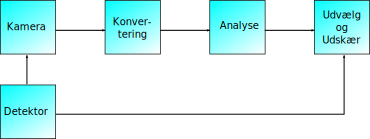
\includegraphics[scale=1]{images/pig-network2}
	\caption{Procesnetværk med detektor til initiering af hvert svin.}
	\label{fig:pig-network2}
\end{center}
\end{figure}

Et problem ved at implementere hele slagterieksemplet i \pycsp er  grænsefladen mellem verden hvor grisene kører på transportbåndet, og  greenletsversionen,  hvor  kun en proces kan være aktiv af gangen. Konvertering og analyse processen arbejder, mens  udskæringsprocessen venter på at svinene kommer inden for rækkevidde. Konvertering- og analysenprocessen  skal dog frivilligt afgive kontrollen, mens svinet er indenfor robottens rækkevidden og hvis de ikke gør, bliver svinet ikke udskåret. I stedet for at det samme system både skal foretage analysen som  styrer robotten, kan vi antage at processerne er mere autonome i deres opbygning. Dette giver at computeren der styrer robotten fungere uafhængigt af de computere der foretager konvertering og analysen. de to computere kan udveksle data igennem f.eks en database, harddisk eller anden delt datastruktur. Hvis analysen bliver færdig gemmes den, i den delte datastruktur, og robotten kan udnytte analysen, Hvis ikke den er klar bruges standard modellen.    



%\subsection{Eksempel 2 - Sensornetværk med høj/lav -prioritet}
%\inline{eks2: skal vise alternation, kan være en sensor som modtager måledata med lav prioritet og som skal sende måledata på opdordring med høj prioritet.}


\section{Design og implementering}
%\inline{Beskrivelse af design med udgangspunkt i eksemplet}
For at designe en implementering af simulering i diskret tid i \pycsp, skal vi foretage en række ændringer i forhold til den nuværende implementering. Specifikt skal vi ændre på planlægningen og eksekveringen af processer, hvortil vi har brug for at kunne repræsentere en diskret tidsmodel. Vi vil i dette afsnit gennemgå de relevante problemstillinger og løsningsmodeller samt give et overblik over, hvordan vi har valgt at implementere ændringerne rent praktisk i koden. 


\subsection{Kodestruktur}  
Efter i kapitel \ref{chap:csp} at have valgt at udvide \emph{greenlets}"-versionen, skal vi vælge hvordan vi ønsker at videreudvikle koden. Vi forventer at genbruge store dele af koden fra \emph{greenlets}"-versionen, og kun foretage udvidelser på enkelte afgrænsede områder. Desuden ønsker vi at isolere vores ændringer fra den originale \emph{greenlets}"-version. Med denne isolation forventer vi, at hvis/når der sker tilrettelser af \emph{greenlets}"-versionen af \pycsp, vil man ikke skulle foretage de samme tilrettelser i vores version. 
Isolationen mellem de to versioner skal opnås via nedarvning, således at det fra en brugers synsvinkel ser ud til, at vores version er fuldstændigt sepereret fra \emph{greenlets}"-versionen.

Hver af de tre versioner har sin egen mappe i \pycsp og i hver af disse findes en tilhørende \code{\_\_init\_\_.py} fil, der fungerer som et manifest for den givne version. Vi opretter vores egen version kaldet \emph{simulation} og opretter også en tilhørende mappe på samme niveau som de andre versioner og med sin egen manifestfil. Manifestfilen kan nu bruges til at udvælge de funktioner, der skal tages direkte fra \emph{greenlets}-versionen, og hvilke funktioner, der skal udvides og som derfor vil ligge i den nye mappe.

\begin{lstlisting}[float=hbtp,label=fig:init,caption=Uddrag af \code{\_\_init\_\_.py} for simulationsversionen.]
from guard import Timeout, Skip
from pycsp.greenlets.alternation import choice
from alternation import Alternation
from pycsp.greenlets.channel import ChannelPoisonException, ChannelRetireException
\end{lstlisting}

I \cref{fig:init} kan man se, at funktionerne \code{choice}, \code{ChannelPoisonException} og \code{ChannelRetireException} alle bliver hentet fra \emph{greenlets}"-versionen, mens funktionerne \code{Timeout, Skip} og \code{Alternation} bliver importeret fra samme mappe og derfor er modificerede versioner. For slutbrugeren  vil dette dog ikke være synligt, og han vil blot se \emph{simulation}"-versionen som en selvstændig version på lige fod med de andre tre versioner.

\subsection{\code{Scheduler}-klassen}
\label{sec:scheduler}
Med valget af \code{greenlets}"-versionen som grundversion, og med henblik på at hovedparten af vores ændringer vil være i \sched en, vil vi kort gennemgå dele af klassen \code{Scheduler}.

\begin{lstlisting}[firstnumber=132,stepnumber=5,numbers=left, float, label=fig:scheduling, caption=Uddrag af Scheduler.py i \emph{greenlets}versionen.]
    def getInstance(cls, *args, **kargs):
        '''Static method to have a reference to **THE UNIQUE** instance'''
        if cls.__instance is None:
            # (Some exception may be thrown...)
            # Initialize **the unique** instance
            cls.__instance = object.__new__(cls)

            # Initialize members for scheduler
            cls.__instance.new = []
            cls.__instance.next = []
            cls.__instance.current = None
            cls.__instance.greenlet = greenlet.getcurrent()

            # Timer specific  value = (activation time, process)
            # On update we do a sort based on the activation time
            cls.__instance.timers = []

            # Io specific
            cls.__instance.cond = threading.Condition()
            cls.__instance.blocking = 0
\end{lstlisting}

 I \cref{fig:scheduling} ses et uddrag af initialiseringskoden, der er interessant, fordi det er her alle de interne datastrukturer oprettes. Man kan her se de tre lister af processer, som \sched en har til rådighed til at varetage processkifte. 
 \begin{list}
 \tightlist 
 \item \code{new}: Initieres på linje 140 og består af processer, som lige er blevet planlagt for første gang. Nye processer kan ankomme til listen \code{new} via funktionerne \code{Parallel, Sequence} og \code{Spawn}.
 \item \code{next}: Initieres på linje 141 og indeholder de processer, der er klar til at blive kørt, og som har været kørt på et tidligere tidspunkt. Et eksempel kunne være en proces, der har stoppet sin kørsel for at vente på kommunikation. Processen vil blive placeret i denne liste, når kommunikationen er overstået. 
 \item \code{timers}: Initieres på linje 147 og indeholder de processer, der har tilknyttet en timeout. De skal først planlægges på et senere tidspunkt og venter dermed blot. Hvert element i listen består både af processen samt et tidsstempel for hvornår processen skal genaktiveres. 
 \item \code{blocking}: Initieres på linje 151 og er en variabel. Processer, der venter på IO-operationer, er ikke klar til at blive planlagt, men heller ikke afsluttet. \Sched en kan derfor ikke planlægge dem, men holder styr på antallet af ventende processer vha. denne variabel. Dette bruges bla. for at kunne afgøre om \sched en har planlagt alle processer.
\end{list}

Når \sched en er startet, gennemløber den alle tre lister gentagne gange, indtil de alle er tomme, og der ikke er nogle processer, der er blokeret. Dette betyder at der ikke længere kan komme nye processer til der ønsker at blive lagt på \sched en, og dermed kan den afslutte.

For at markere at vi ikke kun skal  planlægge rækkefølgen
af processerne, men også styre tiden, har vi lavet en
\code{Simulation}"-klasse, der arver fra \code{Scheduler}"-klassen. Alle ændringer
vi skal foretage for at kunne planlægge processer under hensyntagen til tid, vil således være indkapslet i denne klasse. 
Dette har yderligere den fordel, at man tydeligt kan se at alle klasserne i \code{simulation}-versionen arver en \sched~ fra \code{Simulation} og
ikke en \sched \xspace fra \code{greenlets}-versionen.

\subsection{Tid} \label{sec:tid}
For at kunne planlægge begivenheder i \des kræves det at alle processer og \sched en har en global forståelse af tid.  Det er derfor en af hjørnestenene i implementeringen af \des, hvordan tid introduceres til \pycsp.  
Begrebet tid er ikke en del af \csp, men er alligevel blevet introduceret i \pycsp, for  at  kunne tilknytte en timeout til en \code{alternation}. Vi ønsker
at videreudvikle denne struktur til at håndtere tid generelt for alle
processer, og til at fungere med vores tidsmodel, modsat den eksisterende
løsning, hvor \code{time}-modulet benyttes.
 
\CRef{Timeout} viser et eksempel på brugen af tid i det eksisterende \pycsp, hvor en \code{alternation} er villig
til at læse fra kanalenden \code{Cin} i 0,5 sekunder. Hvis ikke der
er modtaget en besked indenfor 0,5 sekunder, accepteres dens \code{timeout-guard},
og processen fortsætter sin kørsel uden at have læst fra kanalen.

\begin{lstlisting}[float=hbtp, 
label=Timeout,caption=Timeout i Alternation (fra dokumentationen til PyCSP)]
Alternation([{Timeout(seconds=0.5):None}, 
             {Cin:None}]).select()
\end{lstlisting}

Fra en brugers synsvinkel repræsenteres tiden internt i \pycsp som realtid, men dette er ikke korrekt. Helt generelt kan computere ikke håndtere kontinuerlige begreber, som realtid er, og \code{time}-modulet, der står for håndtering af tid i Python og dermed \pycsp, kan derfor ikke give brugeren mulighed for at benytte realtid. 

 I stedet tilbyder \code{time}-modulet det, vi vil kalde ``pseudo realtid'', der minder om realtid, men på en række områder afviger fra denne. Den største forskel mellem realtid og pseudo realtid er, at i computere kan tiden ikke være kontinuerlig, men må nødvendigvis være diskritiseret, og som oftest i et fast lille tidsskridt. Vi skal med vores diskrete tidsmodel derfor ikke foretage en konvertering fra kontinuerlig til diskret tid, men i stedet skal foretage en konvertering fra en diskret tidsmodel. hvor tiden stiger med et fast tidsskridt, til en diskret tidsmodel, hvor tiden stiger med variable tidsskridt. Vi skal desuden ændre fremskrivningen af tiden så den  drives af begivenheder og ikke af et eksternt modul, som i pseudo realtid. \fxnote{Kan vi ryste noget ud med hvorfor det er godt vi ikke skal gå fra kontinuerlig til diskret tid?}
 
 
\subsubsection{Sammenhæng mellem tidsintervaller i realtid og diskret tid}
Da man i \code{time}-modulet har et fast tidsskridt, og
realtiden også er inddelt i faste størrelser
som eks. sekunder, kan man med \code{time}-modulet måle tidsintervaller, der
korresponderer med realtiden. I \des findes der ikke en
sammenhæng til  realtiden, da tiden blot er et tal, der starter som 0, og stiger
i arbitrære tidskridt. Når tiden i \des på denne måde er afkoblet
en relation til realtid, giver det ikke mening at have elementer i simuleringen, der er afhængige af realtid. 
I \pycsp kan man planlægge en timeout til at ske om f.eks. 5 sekunder. I \des findes sekunder som
begreb ikke, men man  angiver i stedet, at når tiden er talt op med 5 tidsskridt, skal
begivenheden ske. Der findes dog ikke en total afkobling mellem tiden i \des og realtiden, for givet et konkret problem, der skal modelleres i \des, vil der altid være en sammenhæng mellem tiderne. Men da denne sammenhæng ikke er fast, skal den defineres eksplicit af brugeren, som f.eks at 5 sekunder i problemet defineres som en stigning i tiden med f.eks 5, 0,5 eller 0,05 i simuleringsmodellen.

Når tiden i \des er uafhængig af realtiden, er der ingen grund til at bruge en kompleks model af tiden, og vi har derfor valgt at repræsentere tiden som et positivt tal, der findes internt i \sched en. Dermed findes der kun en version af tiden, da  \sched en er en singelton. For processer, der ønsker at kende tiden, har vi
introduceret funktionen \code{Now}, der returnerer tiden fra \sched en, når funktionen kaldes. En fordel ved brugen af funktionen \code{Now} som en wrapperfunktion til at bede om tiden i forhold til den eksisterende kode, der direkte kalder \code{time}-modulet, er, at vi frigøres fra en konkret implementering af tid. For fremtiden er det kun funktionen \code{Now}, der skal omskrives, for at hele systemet bruger en anden implementering tid.

I den eksisterende kode har det ikke været tiltænkt, at man ønskede at udskifte implementeringen af tiden, vi skal derfor ændre de steder, hvor \code{time}"-modulet er refereret. Heldigvis bruges \code{time}-modulet kun ved udvælgelse af processer fra \code{timers}-listen (\cref{fig:green:timer}). 
\begin{figure}[hbtp]
\begin{minipage}[c]{\linewidth}
\begin{lstlisting}[firstnumber=204, label=fig:green:timer, caption=Udvælgelse af proces fra listen timers (fra scheduling.py)]
if self.timers and self.timers[0][0] < time.time():
  _,self.current = self.timers.pop(0)
  self.current.greenlet.switch()
\end{lstlisting}
\end{minipage}
\begin{minipage}[c]{\linewidth}
\begin{lstlisting}[firstnumber=124, label=fig:sim:timer, caption=Udvælgelse af proces fra listen timers (fra simulation.py)]
if self.timers and self.timers[0][0] <= Now():
  assert self.timers[0][0] == Now()
  _,self.current = heapq.heappop(self.timers)
  self.current.greenlet.switch()
\end{lstlisting}
\end{minipage}
\end{figure}
Her sammenlignes på linje 204 tidsværdi for den første proces i \code{timers} med det nuværende tidspunkt givet af \code{time}-modulet.
Hvis det nuværende tidspunkt er større end værdien i \code{timers}, udvælges denne proces til at køre næste gang og fjernes fra listen.
For at planlægge begivenheder præcist, skal processerne kunne eksekveres på et specifikt tidspunkt. Dermed har  \sched en i \code{simulations}-versionen behov for at kunne  styre aktiveringen af processerne på et finere niveau end, hvad der er muligt med \code{greenlets}"-versionen.  
I \code{simulation}"-versionen har vi fuld kontrol over tiden, da  den står stille, mens processerne eksekveres, hvorfor dette ikke er et problem.
Vi  tilføjer den begrænsning, at tiden skal være præcist det, der er angivet i \code{timers}, før processen skal aktiveres, og ikke kun større, som angivet i \code{greenlets}-versionen. \CRef{fig:sim:timer} viser udvælgelsen af en proces fra \code{timers} i \code{simulerings}-versionen ved brug af \code{Now}-funktionen, hvor tidspunktet skal være præcist det som processen har angivet.

\subsubsection{Fremskrivning af tid}
I pseudo realtid drives tiden frem af et eksternt modul for at efterligne realtid, der kontinuerligt stiger. I pseudo realtid fremskrives tiden derfor uafhængigt af processernes tilstand og derfor vil et program der med korte mellemrum beder om tiden, få et stigende tidspunkt. I \des  skal tiden i modsætning til realtid stå stille, når processerne er aktive, og kun i forbindelse med en planlagt begivenhed skal tiden drives frem til tidspunktet for denne begivenhed.

\fxnote*{skriv tegning}{Vi kan demonstrere, hvordan den kontinuerlige tid har indflydelse på  \pycsp med et eksempel}. Proces 1 har startet en ny tråd via \code{io-decoratoren} og er derfor blokeret. Proces 2 står i en \code{alternation} med en \code{timeout-guard}. Uafhængigt af den tid, det tager proces 1 at komme ud fra sit blokerede kald, skal proces 2 vide hvornår dens timeout er indtrådt. Dette er implementeret i \code{greenlets}-versionen i \cref{fig:blocking_sleep} på linjerne 242 til 251. Her startes en separat tråd, der vil signalere til \sched en, når tiden for næste begivenhed i \code{timers} listen indtræffer. \Sched en kan nu nøjes med at vente på et signal, som vil komme fra enten en blokeret proces eller den nyoprettede tråd.

Når tiden i \des ikke er drevet af en eksternt modul, er nødvendigheden af en ekstra tråd til  håndtering af tid irrelevant. Først når alle begivenheder til et tidsskridt er eksekveret, skal tiden i \des tælles op. Dette betyder i vores konkrete eksempel, at  så længe proces 1 er blokeret, står tiden stille, og  \sched en venter på dem. Vi kan ikke tælle tiden op, blot fordi nogle processer er blokeret af \code{io-decoratoren}, ligesom vi ikke kan tælle tiden op, så længe der er processer der er aktive. %blot mens nogle processer eksekvere en anden tilfældig funktion.

Først når alle processer venter i enten \code{timers} listen eller på kommunikation, kan der ikke ske flere begivenheder og tiden fremskrives. 
I dette tilfælde  kan \sched en finde tidspunktet for den begivenhed, der ligger tættest på det nuværende tidspunkt,  og springe frem til denne begivenhed. Dette er implementeret i \cref{fig:sim_sleep}.
\begin{figure}[hbtp]
\begin{minipage}[c]{\linewidth}
\begin{lstlisting}[firstnumber=239, label=fig:blocking_sleep, caption=Uddrag af \sched en i \code{Scheduler}]
self.cond.acquire()
if not (self.next or self.new):
    # Waiting on blocking processes or all processes have finished!
    if self.timers:
        # Set timer to lowest activation time
        seconds = self.timers[0][0] - time.time()
        if seconds > 0:
            t = threading.Timer(seconds, self.timer_notify)
            # We don't worry about cancelling, since it makes no 
            # difference if timer_notify is called one more time.
            t.start()
            # Now go to sleep
            self.cond.wait()
    elif self.blocking > 0:
        # Now go to sleep
        self.cond.wait()
    else:
        # Execution finished!
        self.cond.release()
        return
self.cond.release()
\end{lstlisting}
\end{minipage}
\begin{minipage}[c]{\linewidth}
\begin{lstlisting}[firstnumber=158, label=fig:sim_sleep, caption= Uddrag af \sched en i \code{Simulation}]
self.cond.acquire()
if not (self.next or self.new):
  # Waiting on blocking processes
  if self.blocking > 0:
    # Now go to sleep
    self.cond.wait()
  #If there exist only processes in timers we can increment
  elif  not (self.next or self.new or self.blocking): 
      if self.timers:
          # inc timer to lowest activation time
          self._t = self.timers[0][0]
      else:
          # Execution finished!
          self.cond.release()
          return
self.cond.release()  
\end{lstlisting}
\end{minipage}
\end{figure}


\subsubsection{Timeout} 
I \pycsp findes der, som nævnt i \autoref{chap:csp} en \code{alternation}, hvor brugeren har mulighed for at tilknytte to specielle guards. Den ene er en SKIP-guard, der giver mulighed for at kommunikere, hvis kanalen er klar, og ellers fortsætte uden at kommunikere. Den anden er timeout-guarden, der udvider SKIP-guarden, så man venter på kommunikation i en given periode, hvorefter man tager SKIP-guarden. 
Når \des indføres, ændres tiden, så timeout-guarden opererer på tidsskridt fremfor en tidsperiode. Vi går derved fra en situation hvor en timeout-guard f.eks. er villig til at vente i fem sekunder, til en situation hvor den er villig til at vente i 5 tidsskridt. Denne ændring virker umiddelbart simpel, men introducerer et problem i forhold til hvornår timeout-guarden vælges: En proces kan nu ønske at kommunikere i indeværende tidsskridt, men ikke i det efterfølgende. Vi kan dog ikke i tidsskridtet evaluere om kommunikation er muligt. Dette skyldes, at tiden står stille, mens processerne er aktive, så selvom kommunikation ikke er muligt på ét tidspunkt i tidsskridtet, så kan en efterfølgende begivenhed i samme tidsskridt muliggøre kommunikation.


En løsningsmodel på denne problemstilling kunne være at lade processer i timeout-guards vente helt frem til næste tidsskridt, og så her lade dem vælge SKIP-guarden. Dette efterfølgende tidsskridt kan enten være et ekstra skridt, vi introducerer specifikt for at håndtere disse timeout-guards, eller det kan være det næste tidsskridt, hvortil der er planlagt en begivenhed. 
Såfremt vi introducerer et kunstigt tidsskridt, skal dette specificeres i definitionen af timeout-guarden. Uanset hvor lille et tidsskridt vi specificerer, kan vi ikke garantere, at der ikke efterfølgende i samme tidsskridt vil blive planlagt en begivenhed, der skal indtræffe mellem indeværende tidsskridt og det kunstige tidsskridt, vi specificerede i timeout-guarden. Herved er der risiko for, at rækkefølgen af begivenheder, der skal udføres, bliver ændret, hvilket er uacceptabelt. 
Alternativt kan man vælge at lade tiden springe til den næste begivenhed, der er planlagt, og der som det første vælge SKIP-guarden. Her vil man ikke risikere at ændre på rækkefølgen, men derimod at springe for langt frem i tiden. Dette kan være et problem, hvis en proces, der tager en SKIP-guard, efterfølgende planlægger en begivenhed.
Begge muligheder har grundlæggende den svaghed, at oprindeligt ønskede man kun at kommunikere i det indeværende tidsskridt og ikke i hverken et vilkårligt lille tidsrum eller i et tilfældigt tidsrum frem til en efterfølgende begivenhed.

En sidste løsningsmodel er at vente til lige før, tiden tælles op, og der kalde de ventende processers SKIP-guards. 
For at kunne adskille hvilke processer, der har en begivenhed til et tidsskridt, og hvilke, der venter på kommunikation, kan vi \fxnote*{illustration}{benytte os af edge-triggering} til at dele hvert tidsskridt op i to grupper, henholdsvis wake-first og wake-last.
I wake-first-gruppen udføres de processer, der har tilknyttet en begivenhed til det givne tidsskridt, mens man i  wake-last-gruppen aktiverer SKIP-guarden for de processer, der venter på en timeout.

Edge-triggering er den bedste løsningsmodel af de beskrevne, da man her har mulighed for at udføre alle begivenheder, som måske resulterer i kommunikation, og først derefter aktivere SKIP-guards for de processer, der har en timeout til samme tidsskridt. Ulempen ved denne metode er at det kræver en mere kompleks implementering, da der nu findes to seperate måder at vente for hhv. begivenheder og timeouts.

\subsection{Funktionen \code{Wait}}\label{sec:Wait}
Vi har valgt at anskue planlægningen af en begivenhed til et bestemt tidspunkt, sådan at den proces der skal udføre begivenheden venter indtil tiden for begivnheden er nået, og først her begynde udførslen. Dette vil i praksis være det samme som en planlægning til tidspunktet men det letter implementeringen da vi ikke behøver nogen viden om specifikke begivenheder i vores \sched. 

\begin{lstlisting}[firstnumber=11 , stepnumber=2, numbers=left,float=hbtp, label=fig:simpy:yield, caption= Et yield i \simpy (taget fra Bank05.py i eksemplet fra \simpy)] 
def visit(self,timeInBank): 
  print now(), self.name," Here I am" 
  yield hold,self,timeInBank print now()
  self.name," I must leave" 
\end{lstlisting}
I programmeringssproget \simpy benytter man også denne metode med at lade en proces vente. Dette gøres ved at
foretage kaldet \code{yield}, som sørger for, at processen ikke
fortsætter, før et defineret tidsrum er gået. \CRef{fig:simpy:yield} viser, at en kunde er ankommet til banken, hvorefter kunden printer tiden, foretager et \code{yield}, printer tiden igen og afslutter.  Når processen har kaldt \code{yield}, er tiden steget med værdien af \code{timeInBank}. Grunden til at \simpy kan bruge \code{yield}, der er indbygget i Python og at dette kald afgiver kontrol over processen i et tidsrum, knytter sig til deres implementering af \simpy, hvor de bruger \code{corutine} som underliggende teknologi. Som standard kan  \code{corutine} afgive kontrollen med en proces via \code{yield}, og \simpy behøver derfor kun at sikre, at tiden er talt tilstrækkeligt op, før de returnerer til processen.

 Vi ønsker i \pycsp at have en lignende mulighed for at lade en proces vente. Med \code{greenlet}-modulet af brugertråde kan vi ikke bruge \code{yield}, da denne er specifik for \code{co-rutines}, men funktionaliteten er allerede delvist introduceret via \code{timeout} til \code{alternation} i \emph{greenlets}-versionen af \pycsp. Vi kan derfor bygge videre på denne funktionalitet med funktionen \code{Wait}, der fungerer som timeout, men som kan kaldes af processerne på et vilkårligt tidspunkt.

\begin{lstlisting}[firstnumber=20,float=hbtp, label=fig:wait, caption=Wait i \code{simulering}-versionen.] 
def Wait(seconds):
  Simulation().timer_wait(Simulation().current, seconds)
  t = Now()+seconds
  while Now()<t:
    p = Simulation().getNext() 
    p.greenlet.switch()
\end{lstlisting}

Funktionen \code{Wait} står for at kalde den interne funktion, der er lavet til timeouts, kaldet timer\_wait, hvorved processen lægges i \code{timers}-listen, og herefter sørge for først at returnere, når tiden er steget til det krævede. \code{Wait} er reelt det eneste værktøj, der skal til for at vente, og dermed planlægge begivenheder ud i fremtiden, og vi har på nuværenede tidspunkt en simpel \des, der kører i realtid. 

\subsection{Timers}  
I \pycsp bruges listen \code{timers} til at placere processer, der venter på en timeout i \code{alternation}. Dette er en niche feature ved \pycsp, som  sjældent bruges, og hvor der sjældent er samlet mange processer på en gang. 
I \cref{sec:Wait} beskriver vi hvordan processer, der ønsker at vente lægges på \code{timers}-listen, og i \cref{sec:tid} beskriver vi, hvordan \sched en kun tæller tiden op, når ingen processer kan foretage sig mere i et givent tidsskridt. Når tiden tælles op, vil  alle processer enten vente på kommunikation eller befinde sig i listen \code{timers}. De processer, der venter i en \code{alternation} og har tilknyttet en timeout, ligger begge steder. Gennemsnitslængden af listen vil derfor stige voldsomt og i vores version og dermed ændres kravene til hvilken  datastruktur der er bedst egnet. 
Med en kort, sjældent brugt liste vil omkostningerne til oprettelse og vedligeholdelse af en avanceret datastruktur være større end fordelene. Til vores skemaplanlægning  vil en min"-hob være det åbenlyse valg, da  man kan  indsætte elementer i konstant tid og fjerne det mindste element i $O(log\ n)$. Skemaplanlægning er specifikt nævnt i introduktionen til Pythons implementering\footnote{\url{http://docs.python.org/dev/3.0/library/heapq.html}} som eksempel på anvendelsesmulighederne for en hob. 

Da implementeringen af en hob allerede findes i Python i modulet \code{heapq}, som er effektivt implementeret i C, vælger vi at bruge denne. Den eneste handling,
der ikke er implementeret som standard, er fjernelsen af et arbitrært element fra hoben. Dette sker i den eksisterende løsning, når en proces
aktiverer et andet valg i \code{alternation} end timeout. I dette tilfælde skal
processen ikke vente på sin timeout, og derfor skal elementet fjernes fra \code{timers} listen. Her må man, som i
en normal liste, lave en lineær søgning i hoben og derefter genoprette
hob"-egenskaben i listen. Det vil dog ikke tage længere tid, da fjernelse af en timeout i \emph{greenlets}"-versionen på nuværende
tidspunkt bruger en lineær søgning, til at finde elementet der skal
fjernes, og genoprettelsen af hob"-egenskaben også kan gøres i lineær tid.

Det kræver ikke meget omskrivning for at konvertere en liste til en hob, hvilket ses ved at sammenligne \cref{fig:green:timer} linje 205 med \cref{fig:sim:timer} linje 126. 

\subsection{Annekteret kode fra \simpy.}
I vores implementering er der en del overlap med \simpy, da det har været en inspirationskilde til hvordan et simuleringssprog kan udvikles i Python. En del af arbejdet med \simpy har vi kunne bruge direkte i vore implementering efter devisen om ikke at genskrive eksisterende god kode. \simpy har en \code{Monitor}-klasse, der kan benyttes til dataindsamling, bearbejdning og visualisering. Denne klasse har vi i stor udstrækning genbrugt. Den fungerer ved at gemme en liste af tid/værdi par. Dermed kan man efter endt simulering, analysere  hvordan værdierne har ændret sig over tid. Klassen \code{Monitor} kan bruges direkte af brugere, hvor de selv  står for at at gemme værdier på passende tidspunkter igennem kørslen af programmet. Man ønsker tit at kende længden af en kø, der som oftest er implementeret via en liste. Vi har derfor lavet vores egen liste der kan indeholde en \code{Monitor}. Når længden af listen ændres, gemmes længden af listen i en montor til brug for senere analyse, uden brugeren selv skal stå det. Alternativt kan man lave en separat proces, hvis eneste formål er med en given frekvens at gemme listens længde. Fordelen ved denne løsning er at intervallet er jævnt fordelt, og man derfor lettere kan foretage tidsspecifik statistik.
 
\section{Evaluering}
  \inline{Evaluering af hvordan eksemplet løses efter den valgte 
  implementering benyttes. Inkluderer test+performance}
\subsection{Test af korrekthed}
  Vi har igennem designet og udviklingen af \code{simulerings}-versionen brugt en Test Driven Development (TDD). I TDD starter man med at skrive tests til en ny egenskab der skal udvikles. Designet er implementeret korrekt når testene kan gennemføres korrekt. Dette medfører at vi løbende i forbindelsen med udviklingen af \emph{simulerings}-versionen har skrevet tests. Desuden har vi integreret alle tests fra \emph{greenlets}-versionen ind i \emph{simulerings}-versionen, således at tests skrevet til \emph{greenlets}-versionen også tester vores version. Resultaterne af testene kan ses i tabel \fxerror{TODO! testene virker ikke:(}
  
\subsection{Eksempler}



\subsection{Effektivitet}  
\inline{skal vi overhoved evaluere performance?}
  


\section{Fremtidigt arbejde}
\section{Opsummering}
